\subsection{Datová analýza}

\begin{figure}[h!]
	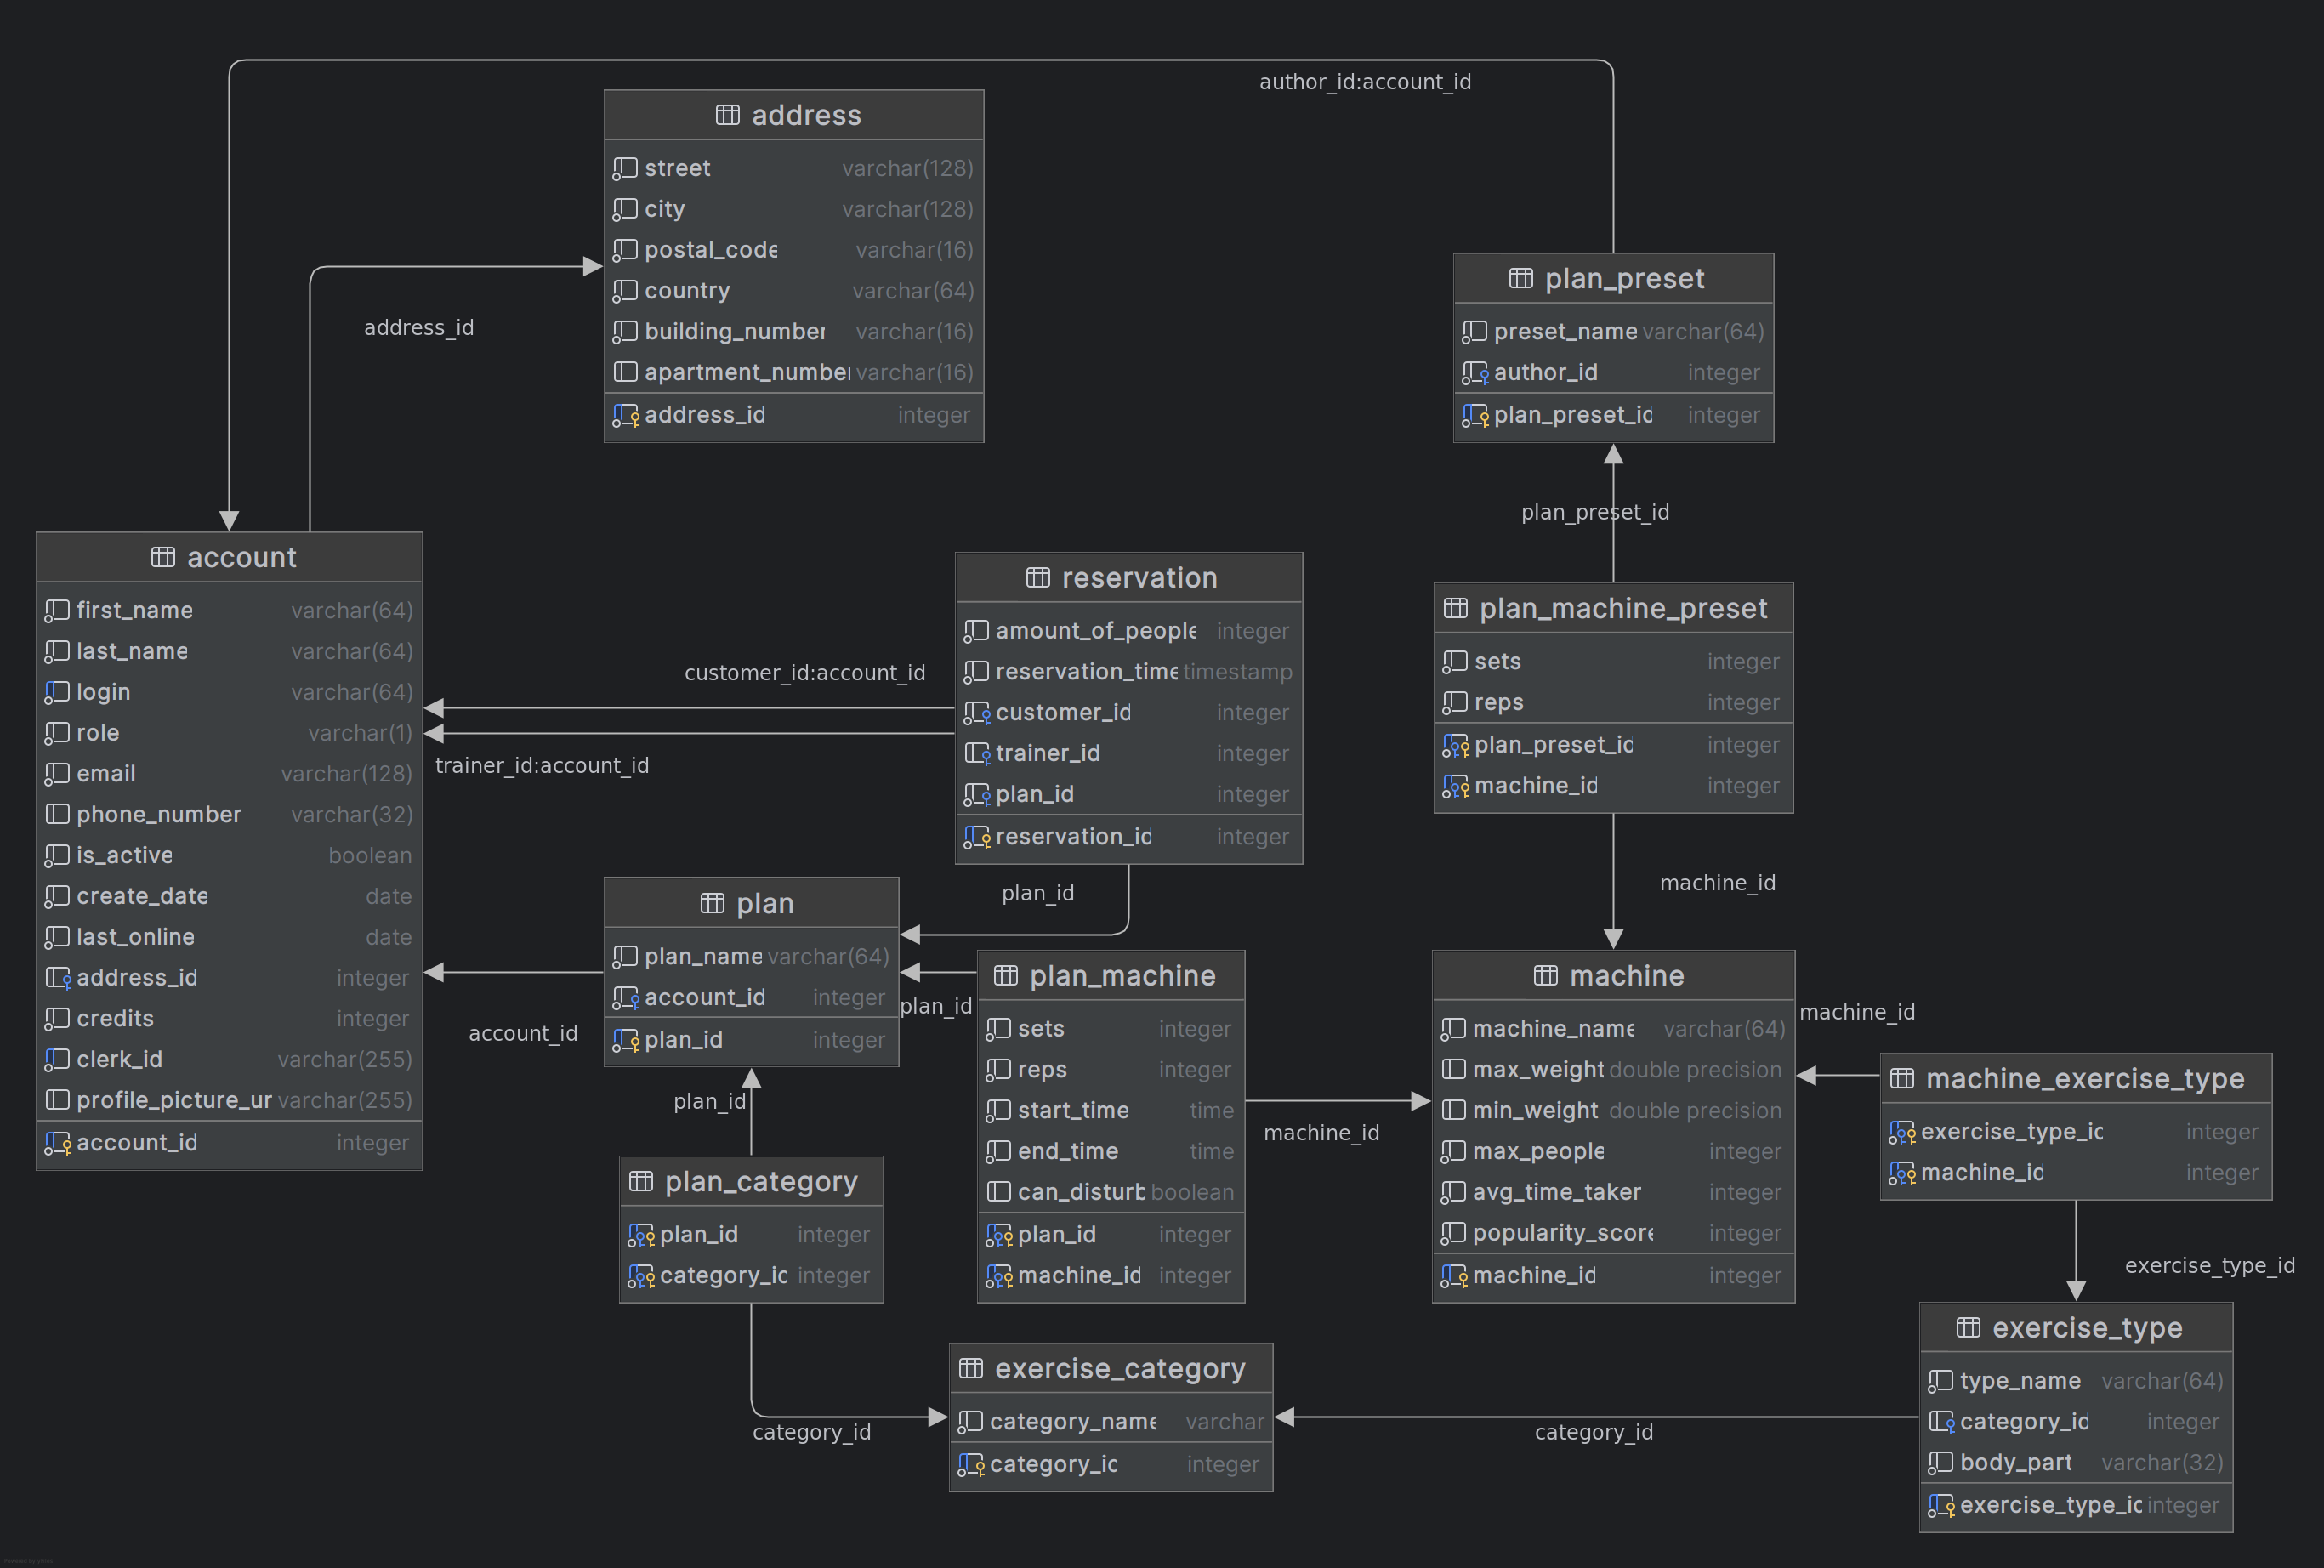
\includegraphics[width=1\textwidth]{Figures/ermodel.png}
	\caption{ Relační model}
	\label{fig:RelationalModel}
\end{figure}

\subsubsection{Popis dat}
Tato sekce se věnuje popisu nejdůležitějších tabulek, které můžeme vidět v ER-modelu. Jedná se o následující 4 tabulky: reservation (rezervace), machine (přístroj), plan (tréninkový plán), plan\_machine (slouží jako vztah mezi přístrojem a plánem, můžeme chápat jako reprezentaci časového okna). Ostatní tabulky slouží primárně k uchovávání doplňujících informací nebo ke správě relací mezi výše uvedenými tabulkami.

\begin{table}[h!]
	\caption{Popis databázové tabulky - reservation}
    \label{tab:dat-dictionary-reservation}
	\begin{tabular}{|p{3.5cm}|p{2cm}|p{1cm}|p{2.5cm}|p{.75cm}|p{3.75cm}|}
		\hline
        \textbf{Název atributu} & \textbf{Dat. Typ} & \textbf{Délka} & \textbf{Klíč} & \textbf{Null} & \textbf{Popis} \\
        \hline
        reservation\_id & INT & - & Primary & Ne & Id rezervace \\
        \hline
        ammout\_of\_people & INT & - & - & Ne & Počet lidí \\
        \hline
        reservation\_time & DATE & - & - & Ne & Čas příchodu \\
        \hline
        customer\_id & INT & - & Cizí (account) & Ne & Id uživatele, na kterého je rezervace napsaná \\
        \hline
        trainer\_id & INT & - & Cizí (account) & Ne & Id trenéra \\
        \hline
        plan\_id & INT & - & Cizí (plan) & Ne & Id plánu \\
        \hline
	\end{tabular}
\end{table}

\begin{table}[h!]
	\caption{Popis databázové tabulky - machine}
    \label{tab:dat-dictionary-machine}
	\begin{tabular}{|p{3.5cm}|p{2cm}|p{1cm}|p{2.5cm}|p{.75cm}|p{3.75cm}|}
		\hline
        \textbf{Název atributu} & \textbf{Dat. Typ} & \textbf{Délka} & \textbf{Klíč} & \textbf{Null} & \textbf{Popis} \\
        \hline
            machine\_id & INTEGER   &  -    & Primary       & Ne & Id stroje \\
            \hline
            machine\_name     & VARCHAR   &  64   & -                 & Ne & Název stroje \\
            \hline
            max\_weight       & FLOAT   &  -   & -                 & Ne &  Maximální váha, kterou lze použít \\
            \hline
            min\_weight       & FLOAT   &  1    & -                 & Ne &  Minimální váha, kterou lze použít \\
            \hline
            max\_people       & INTEGER   &  -  & -                 & Ne & Maximální počet lidí na stroji \\
            \hline
            avg\_time\_taken    & INTEGER   &     & -                 & Ne & Průměrný trávený čas \\
            \hline
            popularity\_score & INTEGER      &  -    & -                 & Ne &  Počet rezervací \\
        \hline
	\end{tabular}
\end{table}

\begin{table}[h!]
	\caption{Popis databázové tabulky - plan}
    \label{tab:dat-dictionary-plan}
	\begin{tabular}{|p{3.5cm}|p{2cm}|p{1cm}|p{2.5cm}|p{.75cm}|p{3.75cm}|}
		\hline
        \textbf{Název atributu} & \textbf{Dat. Typ} & \textbf{Délka} & \textbf{Klíč} & \textbf{Null} & \textbf{Popis} \\
        \hline
            plan\_id & INTEGER   &  -    & Primary       & Ne & Id plánu \\
        \hline
            plan\_name     & VARCHAR   &  64   & -                 & Ne & Název plánu \\
        \hline
            account\_id     & INTEGER   &  -   & -                 & Ne & Id uživatele, který vytvořil plán \\
        \hline
	\end{tabular}
\end{table}

\begin{table}[h!]
	\caption{Popis databázové tabulky - plan\_machine}
    \label{tab:dat-dictionary-plan-machine}
	\begin{tabular}{|p{3.5cm}|p{2cm}|p{1cm}|p{2.5cm}|p{.75cm}|p{3.75cm}|}
		\hline
        \textbf{Název atributu} & \textbf{Dat. Typ} & \textbf{Délka} & \textbf{Klíč} & \textbf{Null} & \textbf{Popis} \\
        \hline
            plan\_id        & INTEGER   &  -    & Cizí (plan)       & Ne & Id plánu \\
        \hline
            machine\_id     & INTEGER   &  -    & Cizí (machine)       & Ne & Id stroje \\
        \hline
            sets                & INTEGER   &  -   & -                 & Ne & TODO \\
        \hline
            reps                & INTEGER   &  -    & -                 & Ne &  TODO \\
            start\_time     & TIME      &  -    & -                 & Ne & Čas začátku \\
        \hline
            end\_time       & TIME      &  -    & -                 & Ne & čas konce \\
        \hline
            can\_disturb          & BOOLEAN   &  1    & -                 & Ne & TODO \\
        \hline
	\end{tabular}
\end{table}

\subsubsection{Procedury a funkce}
Konkrétní procedury a funkce budou popsány v pozdější části této práce. Klíčovým aspektem návrhu je určení, které operace budou efektivnější realizovat na úrovni databáze a které na aplikační vrstvě. Toto rozhodnutí je zásadní, protože ovlivňuje nejen efektivitu a přehlednost řešení, ale také jeho dlouhodobou udržovatelnost.

Procedury a funkce jsou v kontextu navržené architektury využity pro extrakci komplexních datových struktur, nejsou však aplikovány pro jiné operace, jako například manipulace s daty, nebo složitější transakce. Toto rozhodnutí vychází ze dvou východisek:

\begin{description}
    \item[Minimalizace funkcionality databázové vrstvy] 
    Databáze je využita především jako stabilní uložiště dat a optimalizovaný nástroj pro jejich vyhledávání. Transformace dat a obchodní logika je delegována na aplikační vrstvu.
    \item[Využití výhod aplikační vrstvy]
    Výhodou aplikační vrstvy oproti vrstvě datové je možnost využití obecných programovacích jazyků (např. JavaScript), které – na rozdíl od databázového jazyka PL/pgSQL – poskytují širší spektrum nástrojů pro manipulaci s daty, implementaci procedurální logiky a správu komplexních operací.  
\end{description}
Tento přístup přesouvá složitou obchodní logiku z databázové vrstvy do prostředí, které lépe odpovídá požadavkům na moderní softwarový vývoj. Zároveň toto rozhodnutí reflektuje princip separace zodpovědnosti (Separation of Concern - SoC), čímž ustanovuje jasné hranice mezi aplikační a datovou vrstvou, které následně vedou k více robustnímu a bezpečnému řešení. \cite{de2002importance}
